\chapter{Methodology}

\section{Construction Workflow and Phased Development Plan}

Building a combined automotive dealership management platform and consumer-facing e-commerce portal required careful sequencing rather than developing all system components simultaneously. Attempting to build UI-level features before establishing stable database contracts would have created circular dependency problems throughout the codebase. To address this, I structured the entire build around an incremental phased approach where each completed phase served as a stable foundation for the next. This gave me confidence that every endpoint, view, and template was operating against verified data structures from the moment of creation.

The construction workflow progressed across four sequential phases:

\begin{enumerate}
    \item \textbf{Schema Design and Database Normalization:} Starting from the real-world operational structure of multi-branch car dealerships, I mapped out all entities, their relationships, and cardinality constraints. The resulting relational schema, normalized to Third Normal Form ($3\text{NF}$), spans geographic lookup tables (\texttt{Country}, \texttt{City}), operational tables (\texttt{Store}, \texttt{Employee}, \texttt{Employee}\allowbreak\texttt{Hierarchy}), catalog tables (\texttt{Industry}\allowbreak\texttt{Info}, \texttt{Vehicle}\allowbreak\texttt{Info}, \texttt{Inventory}), transaction tables (\texttt{Selling}\allowbreak\texttt{Info}, \texttt{Invoice}, \texttt{Employee}\allowbreak\texttt{Budget}), and customer interaction tables (\texttt{Customer}, \texttt{Customer}\allowbreak\texttt{Info}, \texttt{Customer}\allowbreak\texttt{Message}).
    \item \textbf{ERP Backend Engineering (\texttt{car\_sales}):} With the database schema validated through migration scripts, I built the internal management application. This involved coding the nine-level access control layer, the numeric ID-based authentication backend, all REST API endpoints, and the raw SQL reporting engine that bypasses ORM overhead for executive-facing analytics.
    \item \textbf{Consumer Portal Development (\texttt{ecommerce}):} Using the shared database instance from Phase 2 as a foundation, I constructed the customer-facing application. This included the vehicle catalog and search filter engine, the side-by-side spec comparison tool, wishlist toggling, test-drive booking workflows, and the order checkout pipeline with atomic inventory reservation.
    \item \textbf{Integration, Data Export, and Test Coverage:} The final phase connected both applications over a single database connection and added cross-cutting concerns: JSON and CSV export endpoints, ApexCharts-powered analytics dashboards, and a 21-case automated testing suite covering authentication edge cases, permission boundary enforcement, and inventory concurrency.
\end{enumerate}

Completing migration scripts and populating seed data before any view code was written ensured that every HTTP handler had a predictable, contract-stable data layer to operate against throughout the entire internship project.

\section{System Architecture and Application Partitioning}

The platform is structured around a multi-tier Browser/Server (B/S) separation of concerns. Rather than placing presentation rendering, business rule evaluation, and database access in the same code paths, I separated these responsibilities across distinct architectural layers, consistent with the tier-isolation principles outlined by Junhua~\cite{junhua2011design}. To preserve strict modularity without duplicating shared core entities, the project is partitioned into two distinct Django applications coexisting within a single project workspace.

The first application, \texttt{car\_sales}, handles all internal dealership operations. It owns the primary database schema, manages employee hierarchy tracking, drives inventory logistics, generates sales invoices, calculates selling price variances against Manheim Market Report (MMR) benchmarks, maintains customer messaging inboxes for store-level staff, and powers all executive-facing reporting dashboards. The second application, \texttt{ecommerce}, serves public retail customers by importing shared entity models directly from \texttt{car\_sales} via standard Python imports and extending them with consumer-specific models: \texttt{Wishlist}, \texttt{Cart}, \texttt{CartItem}, \texttt{TestDriveBooking}, \texttt{Order}, and \texttt{PaymentTransaction}. This separation allows both modules to operate against a single database instance without duplicating schema definitions.

Figure~\ref{fig:django_architecture} illustrates the Model-View-Template (MVT) request-response cycle that underpins both applications. Unlike the traditional MVC pattern where a Controller mediates between model and view, Django's MVT architecture assigns that coordination role to the View layer itself. Each incoming browser request is first intercepted by Django's URL dispatcher (\texttt{urls.py}), which matches the request path against registered patterns and routes it to the appropriate view function in \texttt{views.py}. The view function carries all business logic: it queries or mutates data through \texttt{models.py} using the Django ORM, or issues hand-written SQL directly via \texttt{django.db.}\allowbreak\texttt{connection.cursor()} for performance-critical reporting routines. Once the view has assembled its response context, it passes that data to a Template, which renders the final HTML and returns it to the browser. This MVT separation keeps data definitions in Models, processing logic in Views, and presentation concerns exclusively in Templates, making each layer independently testable and maintainable across both the \texttt{car\_sales} and \texttt{ecommerce} applications.

\begin{figure}[H]
\centering
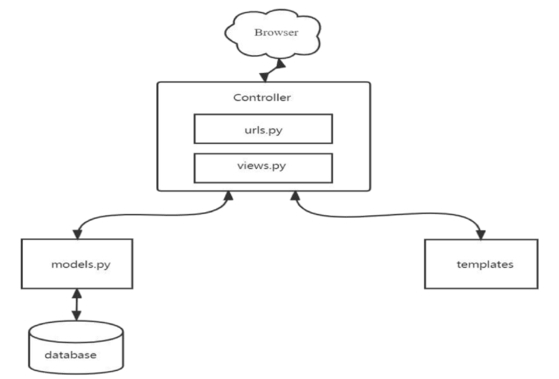
\includegraphics[width=0.85\textwidth]{images/django framework.jpg}
\caption{Django Model-View-Template (MVT) Request-Response Architecture}
\label{fig:django_architecture}
\end{figure}

For the technology stack, I selected Python 3.11 and Django 6.0+ for the backend runtime alongside Django REST Framework (DRF) for structured JSON API responses. On the frontend, I deliberately avoided heavy JavaScript rendering frameworks to keep client-side execution lightweight. All UI pages are rendered server-side using Django's native template engine, with Vanilla CSS stylesheets for layout and targeted JavaScript \texttt{fetch()} calls (AJAX) for asynchronous updates such as wishlist toggling and catalog filter refreshes.

\section{Access Control Architecture and Identity Verification}

Automotive dealership networks operate with clearly defined chains of authority. Corporate executives require visibility across all branches simultaneously, regional directors need access only within their assigned territory, branch-level managers need data scoped to their specific store, and front-line sales representatives should see only records they personally own. Enforcing these boundaries in software required a purpose-built access control layer rather than relying on a generic permission framework.

\subsection{Nine-Level Role Hierarchy}

I designed a nine-level permission hierarchy where each user account is assigned an explicit integer level from 1 to 9. Levels 1 through 5 represent executive tiers (Chief Executive Officer, Vice President of Sales, Operations Director, Financial Controller, and Chief Information Officer) with global read and write privileges across all branches. Level 6 represents regional sales managers responsible for multi-store territories. Levels 7 and 8 represent store managers and assistant managers whose access is restricted to their assigned store location. Level 9 represents individual sales representatives who can only view and edit sale records they created.

In code, this hierarchy is implemented as a custom Django view decorator, \mbox{\texttt{@role\_required}}\allowbreak\texttt{(min\_level)}, applied to protected URL endpoints. When a user requests a view such as \texttt{/car\_sales/}\allowbreak\texttt{dashboard/}, the decorator checks the user's assigned level in \texttt{EmployeeHierarchy}. If the user's level is less than or equal to \texttt{min\_level}, execution proceeds; otherwise, the decorator returns an \texttt{HTTP 403 Forbidden} response immediately.

\subsection{Numeric ID Authentication Backend}

Standard Django authentication expects a username string. However, in retail dealership operations, employees identify themselves by assigned numeric staff IDs. To support this operational pattern, I implemented a custom authentication backend, \mbox{\texttt{EmployeeBackend}}, extending Django's \texttt{ModelBackend}. The custom backend accepts a numeric employee ID and password, verifies the credentials against the hashed password field, checks that the employee's status in \texttt{EmployeeStatus} is active, and populates the request session with the employee's role and branch scope.

\section{Direct SQL Reporting Engine}

During early development, executing Django ORM queries to generate executive financial summaries revealed a measurable performance problem. When aggregating thousands of sales records spanning multiple stores, the ORM constructs verbose SQL JOIN statements and hydrates each database row into a full Python model instance, consuming unnecessary memory and CPU time. Drawing on the analytical database query findings from Vicente et al.~\cite{vicente2021rdbms}, I constructed a parallel reporting layer that executes hand-written SQL statements directly through \texttt{django.db.}\allowbreak\texttt{connection.cursor()}, returning lightweight Python dictionaries without instantiating any model objects.

The engine covers six distinct analytical procedures. The first calculates sales representative performance by grouping \texttt{selling\_info} rows using \texttt{GROUP BY employee\_id} combined with \texttt{SUM()} aggregations to produce per-representative unit volumes and gross revenue totals. The second runs multi-table JOIN aggregations across \texttt{selling\_info}, \texttt{invoice}, and \texttt{store} to compute branch-level revenue totals and average unit selling prices. The third uses dimensional grouping by store location and vehicle make/model to reveal which specific models are performing best at each branch, supporting regional purchasing decisions. The fourth joins \texttt{selling\_info} and \texttt{invoice} by \texttt{customer\_id} to produce total lifetime purchase values per customer account. The fifth detects whether individual customers purchase across multiple store locations, surfacing cross-branch behavioral patterns useful for loyalty programs. The sixth and most complex procedure uses \texttt{CASE WHEN} logic and \texttt{SUM()} aggregations to compare actual monthly revenue per employee against planned targets stored in \texttt{Employee}\allowbreak\texttt{Budget}, computing variance percentages dynamically inside the database engine without round-tripping data to Python.

To accelerate all these queries, I created targeted indexes during migration: \texttt{selling\_date} on \texttt{SellingInfo} is declared with \texttt{db\_index=True}, and \texttt{VehicleInfo} carries an explicit index on the \texttt{make} foreign key. Composite unique constraints on \texttt{Employee}\allowbreak\texttt{Budget} across the fields \texttt{employee}, \texttt{budget\_year}, \texttt{budget\_month}, and \texttt{store} prevent duplicate budget entries and naturally support GROUP BY lookups.

\section{Customer-Facing Catalog and Transaction Pipeline}

Designing the \texttt{ecommerce} application required balancing rich interaction features with execution speed, avoiding the developer-side usability friction associated with heavy off-the-shelf CMS platforms documented by Abdullah et al.~\cite{abdullah2021evaluating}.

\subsection{Catalog Filter and Search Engine}

The vehicle catalog is built around the \texttt{VehicleInfo} schema, which captures make, model, trim, body style, transmission type, VIN, odometer reading, condition score, interior color, and MMR pricing. Rather than implementing a collaborative filtering recommendation engine---which Savadatti and Krishna~\cite{savadatti2024implementation} identified as introducing cold-start latency for new catalog items---I implemented a zero-cold-start filter engine using indexed database queries. Customers interact with filter controls on the catalog page; a client-side JavaScript \texttt{fetch()} call assembles the selected parameters into a structured GET request to the \texttt{/api/vehicles/} endpoint, which queries the database and returns a JSON payload that updates the catalog grid without any page reload.

\subsection{Side-by-Side Vehicle Comparison}

To support purchase decision-making, I engineered a comparison feature that accepts up to four vehicle IDs simultaneously. The comparison view retrieves the full attribute set for each selected vehicle and constructs a comparative matrix covering technical specifications, mileage readings, pricing relative to MMR benchmarks, body type, transmission, and condition grade. Selected vehicles are tracked in browser \texttt{localStorage} so the comparison state persists as the customer navigates across catalog pages.

\subsection{Inventory Reservation and Concurrency Safety}

To prevent two customers from reserving the same vehicle simultaneously, I modeled inventory availability as a formal state machine inside the \texttt{Inventory} model using Django's \texttt{IntegerChoices} where status is defined as \texttt{AVAILABLE (4)}, \texttt{PRE\_ORDER (2)}, \texttt{UNAVAILABLE (0)}, or \texttt{SOLD (1)}. When a customer submits a test-drive booking or a purchase order, the service function wraps the entire reservation sequence inside \texttt{transaction.atomic()}. Within the atomic block, the code verifies that the vehicle's current status is \texttt{AVAILABLE (4)}, transitions it to \texttt{PRE\_ORDER (2)}, links it to the customer record, and commits the change as a single unit. Any concurrent request attempting to reserve the same inventory item will fail the availability check upon reading the already-updated status, preventing duplicate reservations cleanly.

\section{Data Export and Automated Quality Verification}

\subsection{Dual Export Channels}

Two structured export pathways serve different reporting consumers. Custom DRF serializers output clean JSON representations of sales summaries, vehicle catalogs, and staff hierarchy data consumed by the ApexCharts-based analytics dashboards in the \texttt{car\_sales} frontend. Separately, dedicated export view functions utilize Python's built-in \texttt{csv} module to query the raw SQL reporting engine, format the tabular output, and stream a \texttt{Content-Type:}\allowbreak\texttt{text/csv} attachment response directly to the administrator's browser for immediate download without any intermediate file storage step.

\subsection{Automated Test Suite}

To provide empirical verification of system correctness and security, I built a 21-case test suite using Django's \texttt{TestCase} framework inside \texttt{car\_sales/tests.py}. The suite reads seed data from the project Excel dataset via \texttt{pandas}, establishing consistent baseline records without requiring a live production database. For authentication coverage, \mbox{\texttt{EmployeeBackend}} is tested against valid numeric logins, incorrect passwords, non-existent employee IDs, and terminated employee accounts, with each rejection path verified to return \texttt{None} without raising exceptions. For access control coverage, tests assert that Level 9 employees cannot reach executive reporting endpoints, and that Levels 6 through 8 employees are denied DELETE operations with an \texttt{HTTP 403 Forbidden} response. For transaction integrity, integration tests confirm that \texttt{transaction.atomic()} correctly updates inventory status during order placement and that duplicate booking attempts are rejected before any database commit occurs. Finally, all REST endpoints are verified to return the expected HTTP status codes---$200\text{ OK}$, $201\text{ Created}$, and $403\text{ Forbidden}$---along with correct JSON response structures under both authorized and unauthorized request conditions. Running \texttt{python manage.py test} executes all 21 routines against an isolated test database, producing an empirical proof of correctness before any code is deployed.